\documentclass[a4paper,12pt]{article}
% ----- Packages -----
\usepackage[a4paper, margin=1in]{geometry}
\usepackage{graphicx}
\usepackage{titlesec}
\usepackage{fancyhdr}
\usepackage[hidelinks]{hyperref}
\usepackage{amsmath}
\usepackage{enumitem}
\usepackage{lipsum}
\usepackage{parskip}
\usepackage{tikz}
\usepackage{tabularx}
\usepackage{float}
\usepackage{everypage}
\usepackage{mathptmx}
\usepackage[utf8]{inputenc}
\AddEverypageHook{%
  \begin{tikzpicture}[remember picture, overlay]
    \draw[line width=1pt]
      ([xshift=1cm,yshift=-1cm]current page.north west) rectangle
      ([xshift=-1cm,yshift=1cm]current page.south east);
  \end{tikzpicture}
}
% ----- Title Setup -----
\title{}
\author{}
\date{}

% ----- Header/Footer Setup -----
\pagestyle{fancy}
\fancyhf{}
\rhead{Hotel Management SDS}
\lhead{Noel Ninan Sheri}
\cfoot{\thepage}

\begin{document}
\fontsize{13}{16}\selectfont

\begin{titlepage}
\begin{center}
\vspace*{3cm}
\Huge \textbf{Software Design Specification} \\
\vspace{0.5cm}
\LARGE for \\
\vspace{0.5cm}
\Huge \textbf{Hotel Management System} \\

\vspace{3cm}
\Large
Submitted by \\
\vspace{0.3cm}
\textbf{Noel Ninan Sheri} \\
\textbf{23MIS0026} \\
\textbf{School of Computer Science and Engineering Systems} \\
\textbf{Vellore Institute of Technology, Vellore} \\

\vfill
\Large March 2025
\end{center}
\end{titlepage}

% ---- New Page for TOC ----
\newpage
\tableofcontents
\newpage

% ----- SDS Sections -----
\section{Introduction}

The Software Design Specification (SDS) document for the Hotel Management System (HMS) outlines the detailed design and architectural components required to implement a robust, efficient, and user-friendly system. 

This document serves as a bridge between the Software Requirements Specification (SRS) and the actual implementation, providing developers and stakeholders with a technical blueprint for the system.

The Hotel Management System is intended to simplify and automate the day-to-day operations of a hotel such as room bookings, guest check-in/check-out, billing, and reporting. The design emphasizes modularity, scalability, and ease of maintenance, ensuring the system can evolve with future requirements.

The document covers architectural design, data models, interface definitions, component-level designs, user interface considerations, and the overall structure of the software solution.

\section{System Overview}
The Hotel Management System (HMS) is a web-based software solution designed to streamline hotel operations and enhance guest experiences. The system encompasses various modules that work together to automate and manage different aspects of hotel administration.

\subsection*{Key Modules and Responsibilities}

\begin{itemize}
    \item \textbf{Reservation Management:} Handles room booking requests, availability checks, and booking confirmations.
    \item \textbf{Front Desk Operations:} Manages check-in and check-out processes, room assignments, and guest information.
    \item \textbf{Room Management:} Maintains status of rooms (available, occupied, under maintenance), and facilitates room updates.
    \item \textbf{Billing and Invoicing:} Generates bills for guests based on stay, services used, taxes, and discounts.
    \item \textbf{User Management:} Manages roles like admin, receptionist, and housekeeping with authentication and access control.
    \item \textbf{Housekeeping Module:} Tracks cleaning schedules, room service status, and requests from guests.
    \item \textbf{Report Generation:} Provides daily, weekly, and monthly reports on occupancy, revenue, and other KPIs.
\end{itemize}

\subsection*{Users of the System}

\begin{itemize}
    \item \textbf{Admin:} Oversees the entire system, manages users, and views reports.
    \item \textbf{Receptionist:} Handles guest bookings, check-in/check-out, and billing.
    \item \textbf{Housekeeping Staff:} Updates cleaning status and responds to service requests.
    \item \textbf{Guests:} Make reservations and provide feedback.
\end{itemize}

\subsection{Project Goals vs Benefits to Stakeholders}

\begin{table}[H]
\centering
\begin{tabularx}{\textwidth}{|X|X|}
\hline
\textbf{Project Goal} & \textbf{Benefit to Stakeholders} \\
\hline
Automate hotel operations & Hotel staff save time and reduce manual errors \\
\hline
Provide a user-friendly online booking system & Guests can book rooms anytime, anywhere, with ease \\
\hline
Enable secure login and role-based access & Ensures system security for Admin, Staff, and Guests \\
\hline
Maintain structured records of guests, bookings, etc. & Admins can track history, generate reports, and make informed decisions \\
\hline
Generate real-time reports and analytics & Admins get operational insights to improve services \\
\hline
Enable digital payments with receipts & Guests enjoy convenience and transparency; reduces cash handling \\
\hline
Capture guest feedback & Helps management evaluate service quality and improve guest experience \\
\hline
Ensure mobile responsiveness & All users can access the system from phones, tablets, or PCs easily \\
\hline
\end{tabularx}
\caption{Project Goals vs Benefits to Stakeholders}
\end{table}

The use case diagram provides a high-level visualization of how various actors interact with the Hotel Management System. It captures the essential functionalities offered to different types of users such as Admin, Guest, Receptionist, and Housekeeping Staff. Each actor is associated with relevant use cases like booking rooms, managing user accounts, processing payments, handling feedback, and generating reports. The diagram ensures that all user interactions are clearly defined and mapped to specific system functionalities, facilitating a better understanding of the system’s overall behavior. This structured approach also aids in identifying system boundaries and actor responsibilities early in the design phase, promoting clarity and consistency throughout the software development lifecycle.
\subsection{Use Case Diagram}

\begin{figure}[H]
\centering
\begin{tikzpicture}[actor/.style={draw, fill=gray!20, rectangle, minimum height=0.8cm},
                    usecase/.style={draw, ellipse, minimum width=2.5cm, minimum height=1.2cm},
                    line/.style={-latex}]

% Actors
\node[actor] (guest) at (-6, 0) {Guest};
\node[actor] (receptionist) at (-6, -5) {Receptionist};
\node[actor] (admin) at (6, -5) {Admin};

% Use Cases
\node[usecase] (register) at (0, 2.5) {Register};
\node[usecase] (login) at (0, 1) {Login};
\node[usecase] (searchroom) at (0, -0.5) {Search Room};
\node[usecase] (bookroom) at (0, -2) {Book Room};
\node[usecase] (payment) at (0, -3.5) {Make Payment};
\node[usecase] (feedback) at (0, -5) {Submit Feedback};
\node[usecase] (viewbookings) at (-1.5, -6.5) {View Bookings};
\node[usecase] (checkinout) at (-1.5, -8) {Check-In/Out};
\node[usecase] (manageusers) at (3, -6.5) {Manage Users};
\node[usecase] (managerooms) at (3, -8) {Manage Rooms};
\node[usecase] (viewreports) at (3, -9.5) {View Reports};
\node[usecase] (viewfeedback) at (3, -11) {View Feedback};

% Guest links
\draw[line] (guest) -- (register);
\draw[line] (guest) -- (login);
\draw[line] (guest) -- (searchroom);
\draw[line] (guest) -- (bookroom);
\draw[line] (guest) -- (payment);
\draw[line] (guest) -- (feedback);

% Receptionist links
\draw[line] (receptionist) -- (login);
\draw[line] (receptionist) -- (viewbookings);
\draw[line] (receptionist) -- (checkinout);

% Admin links
\draw[line] (admin) -- (login);
\draw[line] (admin) -- (manageusers);
\draw[line] (admin) -- (managerooms);
\draw[line] (admin) -- (viewreports);
\draw[line] (admin) -- (viewfeedback);

\end{tikzpicture}
\caption{Use Case Diagram for Hotel Management System}
\end{figure}

\section{System Architecture}

The Hotel Management System follows a three-tier architecture comprising the Presentation Layer, Business Logic Layer, and Data Layer. This architecture ensures separation of concerns, modularity, and scalability.

\begin{itemize}
    \item \textbf{Presentation Layer:}
    \begin{itemize}
        \item Provides the graphical user interface for users (guests, staff, admin).
        \item Built using HTML, CSS, JavaScript, and Bootstrap for responsiveness.
        \item Communicates with the business logic layer through HTTP requests.
    \end{itemize}

    \item \textbf{Business Logic Layer:}
    \begin{itemize}
        \item Acts as the bridge between the presentation and data layers.
        \item Developed using PHP (or Node.js/Java/Python as alternatives based on deployment).
        \item Handles room allocation logic, booking flow, payment processing, authentication, etc.
    \end{itemize}

    \item \textbf{Data Layer:}
    \begin{itemize}
        \item Consists of a MySQL relational database.
        \item Stores persistent data like user information, room details, bookings, and transactions.
        \item Enforces constraints and maintains referential integrity.
    \end{itemize}
\end{itemize}

The system uses RESTful APIs for communication between client and server. The architecture supports role-based access control to ensure secure and restricted operations. Optional integration with third-party payment gateways (like Razorpay or PayPal) is also supported.

\vspace{0.5cm}
\textbf{Technology Stack:}
\begin{itemize}
    \item \textbf{Frontend:} HTML, CSS, JavaScript, Bootstrap
    \item \textbf{Backend:} PHP (or optionally Node.js/Java/Python)
    \item \textbf{Database:} MySQL
    \item \textbf{Web Server:} Apache or Nginx
\end{itemize}

The architecture diagram below illustrates the layered structure of the Hotel Management System. The system is built using a five-layer model, with each layer having a specific responsibility:

- The **User Interface Layer** consists of components that users interact with, like the Guest and Admin interfaces.
- The **Application Layer** contains modules such as Booking and Feedback, which handle specific user interactions.
- The **Business Logic Layer** performs validation and enforces business rules through dedicated components.
- The **Data Access Layer** serves as a bridge to interact with the database.
- Finally, the **Database Layer** stores all persistent data using MySQL.

This modular design improves scalability, maintainability, and separation of concerns across different parts of the system.
\begin{figure}[H]
\centering
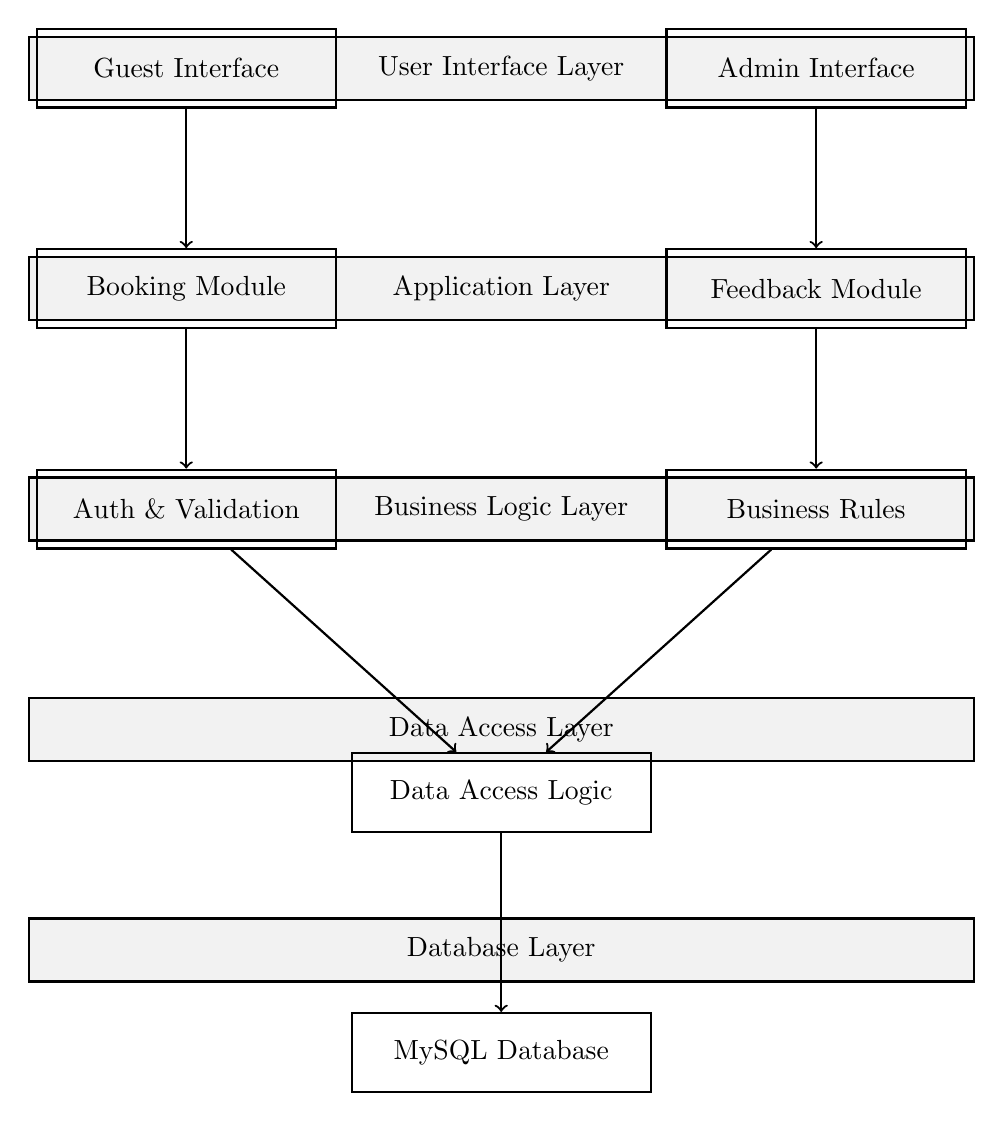
\begin{tikzpicture}[
    component/.style={rectangle, draw=black, thick, minimum width=3.8cm, minimum height=1cm, align=center},
    layer/.style={rectangle, draw=black, fill=gray!10, thick, minimum height=0.8cm, minimum width=12cm, align=center},
    arrow/.style={->, thick}
]

% Layer Headings
\node[layer] at (0,10) (ui) {User Interface Layer};
\node[layer] at (0,7.2) (app) {Application Layer};
\node[layer] at (0,4.4) (biz) {Business Logic Layer};
\node[layer] at (0,1.6) (data) {Data Access Layer};
\node[layer] at (0,-1.2) (db) {Database Layer};

% UI Components
\node[component] at (-4,10) (guestui) {Guest Interface};
\node[component] at (4,10) (adminui) {Admin Interface};

% Application Modules
\node[component] at (-4,7.2) (booking) {Booking Module};
\node[component] at (4,7.2) (feedback) {Feedback Module};

% Business Logic
\node[component] at (-4,4.4) (auth) {Auth \& Validation};
\node[component] at (4,4.4) (rules) {Business Rules};

% Data Access
\node[component] at (0,0.8) (dal) {Data Access Logic};

% Database (already shifted down to avoid overlap)
\node[component] at (0,-2.5) (dbase) {MySQL Database};

% Arrows
\draw[arrow] (guestui) -- (booking);
\draw[arrow] (adminui) -- (feedback);
\draw[arrow] (booking) -- (auth);
\draw[arrow] (feedback) -- (rules);
\draw[arrow] (auth) -- (dal);
\draw[arrow] (rules) -- (dal);
\draw[arrow] (dal) -- (dbase);

\end{tikzpicture}
\caption{Architecture Diagram of Hotel Management System}
\end{figure}

\section{Data Design}
The Hotel Management System uses a relational database model to efficiently manage and store data. The core tables and their primary functions are described below:

\begin{enumerate}
    \item \textbf{Users Table:}
    \begin{itemize}
        \item Stores information about all system users (Admins, Receptionists, Housekeeping Staff, Guests).
        \item Key fields: UserID (Primary Key), Name, Email, Password, Role, Phone.
    \end{itemize}

    \item \textbf{Rooms Table:}
    \begin{itemize}
        \item Stores room details including status, type, and pricing.
        \item Key fields: RoomID (Primary Key), RoomType, PricePerNight, Status (Available/Occupied/Maintenance).
    \end{itemize}

    \item \textbf{Bookings Table:}
    \begin{itemize}
        \item Records all room booking transactions.
        \item Key fields: BookingID (Primary Key), UserID (Foreign Key), RoomID (Foreign Key), CheckInDate, CheckOutDate, TotalAmount, PaymentStatus.
    \end{itemize}

    \item \textbf{Payments Table:}
    \begin{itemize}
        \item Tracks payments for room bookings.
        \item Key fields: PaymentID (Primary Key), BookingID (Foreign Key), PaymentMethod, AmountPaid, PaymentDate.
    \end{itemize}

    \item \textbf{Housekeeping Table:}
    \begin{itemize}
        \item Manages housekeeping schedules and records.
        \item Key fields: TaskID (Primary Key), RoomID (Foreign Key), StaffID (Foreign Key from Users), TaskDate, TaskStatus.
    \end{itemize}
\end{enumerate}

The database design ensures data normalization and referential integrity through the use of primary and foreign keys. Indexing is applied on frequently queried columns for performance optimization.

In addition to the core database schema, the system ensures referential integrity through foreign key constraints and indexes for efficient data access. Data normalization has been considered to reduce redundancy and maintain consistency. Backup strategies and data recovery plans are also in place to safeguard against data loss or corruption.

\section{Modules and Component Design}

The system is divided into several functional modules, each responsible for a specific aspect of hotel management. Each module is encapsulated as an independent component to ensure modularity, maintainability, and scalability.

\subsection{1. User Management Module}
\begin{itemize}
    \item Handles user registration, login, logout, and profile management.
    \item Supports different user roles: Admin, Receptionist, Housekeeping, Guest.
    \item Implements authentication and role-based authorization.
\end{itemize}

\subsection{2. Room Management Module}
\begin{itemize}
    \item Maintains records of all rooms, including room type, price, and availability.
    \item Admin can add, edit, or delete room details.
    \item Automatically updates room status during check-in and check-out.
\end{itemize}

\subsection{3. Booking Module}
\begin{itemize}
    \item Facilitates room booking for guests and staff.
    \item Allows users to check room availability, make a reservation, or cancel bookings.
    \item Updates the availability status in real-time upon confirmation.
\end{itemize}

\subsection{4. Payment Module}
\begin{itemize}
    \item Handles billing and payment processing.
    \item Calculates booking charges including taxes and discounts.
    \item Integrates with third-party payment gateways (e.g., Razorpay, PayPal).
\end{itemize}

\subsection{5. Housekeeping Module}
\begin{itemize}
    \item Tracks cleaning schedules and room status.
    \item Assigns tasks to housekeeping staff.
    \item Allows marking rooms as clean or dirty in real-time.
\end{itemize}

\subsection{6. Reporting Module}
\begin{itemize}
    \item Generates periodic reports for Admin such as occupancy rate, income summary, and housekeeping logs.
    \item Reports can be exported as PDFs or Excel files.
\end{itemize}

\subsection{7. Feedback and Support Module}
\begin{itemize}
    \item Allows guests to leave reviews or request support.
    \item Admin can view and respond to feedback.
\end{itemize}

The Hotel Management System is designed as a modular architecture to promote separation of concerns, reusability, and scalability. Each module is encapsulated as an independent component responsible for a specific business functionality. These modules interact through a centralized Application Controller and communicate with the database via the Data Access Layer. The diagram below illustrates the interconnection of major modules in the system.
\begin{figure}[H]
\centering
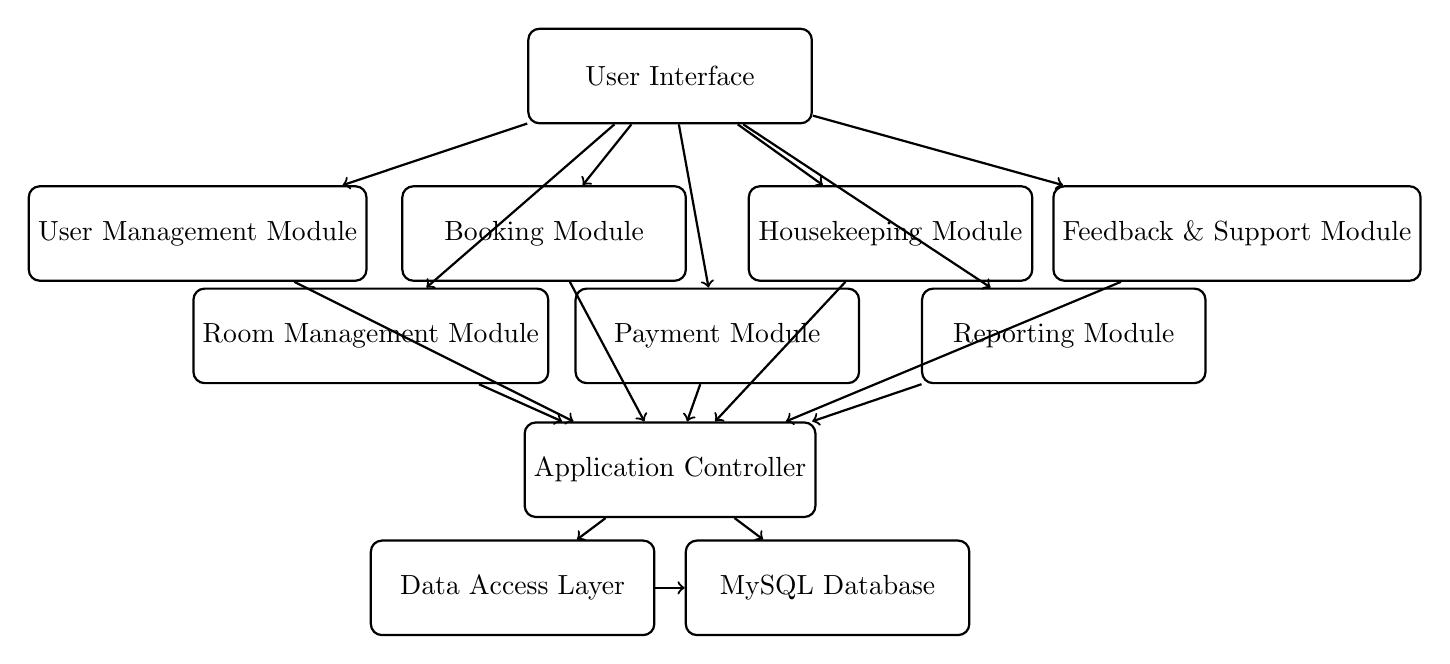
\begin{tikzpicture}[
    component/.style={rectangle, draw=black, thick, rounded corners, minimum width=3.6cm, minimum height=1.2cm, align=center},
    arrow/.style={->, thick}
]

% Top UI Layer
\node[component] at (0,6.5) (ui) {User Interface};

% Middle Modules Layer (spread out 7 modules)
\node[component] at (-6,4.5) (user) {User Management Module};
\node[component] at (-3.8,3.2) (room) {Room Management Module};
\node[component] at (-1.6,4.5) (booking) {Booking Module};
\node[component] at (0.6,3.2) (payment) {Payment Module};
\node[component] at (2.8,4.5) (house) {Housekeeping Module};
\node[component] at (5,3.2) (report) {Reporting Module};
\node[component] at (7.2,4.5) (feedback) {Feedback \& Support Module};

% Controller
\node[component] at (0,1.5) (controller) {Application Controller};

% Data Access + DB
\node[component] at (-2,0) (dal) {Data Access Layer};
\node[component] at (2,0) (db) {MySQL Database};

% Arrows from UI
\draw[arrow] (ui) -- (user);
\draw[arrow] (ui) -- (room);
\draw[arrow] (ui) -- (booking);
\draw[arrow] (ui) -- (payment);
\draw[arrow] (ui) -- (house);
\draw[arrow] (ui) -- (report);
\draw[arrow] (ui) -- (feedback);

% Arrows from Modules to Controller
\draw[arrow] (user) -- (controller);
\draw[arrow] (room) -- (controller);
\draw[arrow] (booking) -- (controller);
\draw[arrow] (payment) -- (controller);
\draw[arrow] (house) -- (controller);
\draw[arrow] (report) -- (controller);
\draw[arrow] (feedback) -- (controller);

% Arrows from Controller to DAL and DB
\draw[arrow] (controller) -- (dal);
\draw[arrow] (controller) -- (db);

% Optional: Connection from DAL to DB (if you prefer)
\draw[arrow] (dal) -- (db);

\end{tikzpicture}
\caption{Modules in Hotel Management System}
\end{figure}


\section{Interface Design}

The Interface Design of the Hotel Management System outlines how different components of the system communicate with each other and with external systems. It focuses on system-level integration, ensuring seamless data exchange and modular connectivity.

\subsection{1. Database Interface}
\begin{itemize}
    \item All modules interact with a centralized relational database (MySQL).
    \item SQL queries are used to fetch, insert, update, and delete records securely.
    \item Prepared statements are employed to prevent SQL injection attacks.
    \item Database schemas are normalized to reduce redundancy and maintain consistency.
\end{itemize}

\subsection{2. Module-to-Module Interfaces}
\begin{itemize}
    \item Modular design enables each functional unit (e.g., Booking, Room Management, Payment) to operate independently yet communicate through defined interfaces.
    \item Function calls and internal APIs facilitate data transfer between modules.
    \item Example: The Booking module sends user and room details to the Payment module for billing.
\end{itemize}

\subsection{3. Admin and Staff Interface}
\begin{itemize}
    \item Role-based authentication ensures restricted access to admin and staff features.
    \item Interface fetches appropriate data views and functionality based on user roles.
    \item Communication with the database and reporting modules is handled through backend APIs.
\end{itemize}

\subsection{4. External Payment Gateway Integration}
\begin{itemize}
    \item Payment module integrates with third-party payment APIs (e.g., Razorpay or Stripe).
    \item Uses secure HTTPS protocols and token-based authentication.
    \item Payment confirmation is captured and relayed to the Booking and Billing modules.
\end{itemize}

\subsection{5. Email Notification System}
\begin{itemize}
    \item The system integrates with an SMTP-based email service.
    \item Booking confirmations, payment receipts, and feedback acknowledgments are sent via automated emails.
    \item Uses templated content with placeholders dynamically replaced by booking/user details.
\end{itemize}

\section{Data Structures}

The following are the key data structures used in the system to represent entities and facilitate various operations:

\subsection{1. User}
\begin{itemize}
    \item \textbf{Fields:} userID, name, email, phoneNumber, role, password
    \item \textbf{Description:} Represents all users including admin, staff, and guests. Stores authentication and profile information.
\end{itemize}

\subsection{2. Room}
\begin{itemize}
    \item \textbf{Fields:} roomID, roomType, price, isAvailable, amenities
    \item \textbf{Description:} Represents each room in the hotel along with availability and pricing details.
\end{itemize}

\subsection{3. Booking}
\begin{itemize}
    \item \textbf{Fields:} bookingID, userID, roomID, checkInDate, checkOutDate, status
    \item \textbf{Description:} Holds all data related to room reservations including dates and user mapping.
\end{itemize}

\subsection{4. Payment}
\begin{itemize}
    \item \textbf{Fields:} paymentID, bookingID, amount, paymentDate, paymentMethod, status
    \item \textbf{Description:} Represents payment details for each booking.
\end{itemize}

\subsection{5. Feedback}
\begin{itemize}
    \item \textbf{Fields:} feedbackID, userID, rating, comment, submissionDate
    \item \textbf{Description:} Captures user feedback for service evaluation and improvement.
\end{itemize}

\subsection{6. Report}
\begin{itemize}
    \item \textbf{Fields:} reportID, type, generatedBy, generationDate, content
    \item \textbf{Description:} Represents summary reports generated by the admin for analytics and insights.
\end{itemize}

\section{Algorithms}

This section outlines the core algorithms used in the Hotel Management System for various functionalities.

\subsection{1. Room Availability Check Algorithm}
\begin{itemize}
    \item \textbf{Input:} Check-in date, Check-out date
    \item \textbf{Output:} List of available rooms
    \item \textbf{Steps:}
    \begin{enumerate}
        \item Retrieve all rooms from the database.
        \item For each room, check if it is already booked during the given date range.
        \item If not booked, mark the room as available.
        \item Return the list of available rooms.
    \end{enumerate}
\end{itemize}

\subsection{2. Booking Confirmation Algorithm}
\begin{itemize}
    \item \textbf{Input:} Room ID, User ID, Check-in date, Check-out date
    \item \textbf{Output:} Booking status
    \item \textbf{Steps:}
    \begin{enumerate}
        \item Validate user credentials.
        \item Check if the selected room is available.
        \item If available, create a new booking record.
        \item Update room availability status.
        \item Send booking confirmation to user.
    \end{enumerate}
\end{itemize}

\subsection{3. Payment Processing Algorithm}
\begin{itemize}
    \item \textbf{Input:} Booking ID, Amount, Payment Method
    \item \textbf{Output:} Payment confirmation
    \item \textbf{Steps:}
    \begin{enumerate}
        \item Validate booking and amount.
        \item Process payment via selected payment gateway.
        \item On success, update payment status in database.
        \item Generate receipt and notify user.
    \end{enumerate}
\end{itemize}

\subsection{4. Feedback Analysis Algorithm (Basic)}
\begin{itemize}
    \item \textbf{Input:} Collection of feedback ratings
    \item \textbf{Output:} Average rating, most common issues (if comments are analyzed)
    \item \textbf{Steps:}
    \begin{enumerate}
        \item Retrieve all feedback entries.
        \item Calculate average rating.
        \item (Optional) Perform keyword search or basic sentiment analysis on comments.
        \item Display overall feedback summary.
    \end{enumerate}
\end{itemize}

\section{User Interface Design}

The user interface (UI) of the Hotel Management System is designed to be intuitive, responsive, and accessible to users with varying technical expertise. It ensures efficient navigation and seamless interaction across different modules.

\subsection{1. Login and Registration Screens}
\begin{itemize}
    \item A clean login screen for returning users with fields for username and password.
    \item Registration interface allows new users (guests) to sign up with required details.
    \item Admin and staff are pre-registered and provided credentials by the system.
\end{itemize}

\subsection{2. Dashboard}
\begin{itemize}
    \item Dynamic dashboard based on user role.
    \item Admin dashboard displays system stats, recent bookings, and reports.
    \item Receptionist dashboard highlights current check-ins/check-outs.
\end{itemize}

\subsection{3. Room Booking Interface}
\begin{itemize}
    \item Shows real-time room availability with filtering options (date, type, price).
    \item Booking confirmation with booking ID and email notification.
\end{itemize}

\subsection{4. Room Management Interface}
\begin{itemize}
    \item Admin interface to add, update, or delete rooms.
    \item Includes room list, occupancy status, and pricing controls.
\end{itemize}

\subsection{5. Payment Interface}
\begin{itemize}
    \item Simple and secure payment screen.
    \item Displays itemized billing before final payment.
    \item Integrates third-party gateways and allows receipt download.
\end{itemize}

\subsection{6. Feedback Form}
\begin{itemize}
    \item Guests can rate their stay and leave comments.
    \item Admin can view all feedback for service improvement.
\end{itemize}

\subsection{7. Mobile Responsiveness}
\begin{itemize}
    \item The interface is designed using responsive design principles.
    \item Accessible on desktops, tablets, and smartphones.
\end{itemize}

The wireframe illustrates the Admin Dashboard layout, showcasing key modules like Bookings, Payments, Rooms, and Reports. It helps visualize content structure, navigation flow, and component placement before full UI development. This layout ensures a clean, user-friendly experience and supports efficient hotel management operations.
\begin{figure}[H]
\centering
\begin{tikzpicture}[every node/.style={draw, minimum height=1cm, anchor=north west}, font=\small]

% Sidebar
\node[fill=gray!20, minimum width=3cm, minimum height=13cm] (sidebar) at (0,0) { 
  \begin{minipage}[t]{3cm}
  \textbf{Sidebar}\\
  \vspace{0.2cm}
  - Dashboard\\
  - Rooms\\
  - Bookings\\
  - Payments\\
  - Housekeeping\\
  - Reports\\
  - Feedback
  \end{minipage}
};

% Header
\node[fill=blue!20, minimum width=12cm, minimum height=1.5cm] (header) at (3,0) {
  \begin{minipage}[t]{12cm}
  \textbf{Admin Dashboard} \hfill [User Icon]
  \end{minipage}
};

% Content Boxes
\node[fill=white, minimum width=5.5cm] at (3,-1.5) {Total Rooms: 60};
\node[fill=white, minimum width=5.5cm] at (9,-1.5) {Bookings Today: 12};

\node[fill=white, minimum width=5.5cm] at (3,-3) {Revenue Today: ₹ 15,000};
\node[fill=white, minimum width=5.5cm] at (9,-3) {Pending Payments: 3};

% Chart area
\node[fill=gray!10, minimum width=11.5cm, minimum height=5.5cm] at (3,-5) {
  \begin{minipage}[t]{11.5cm}
  \textbf{Occupancy Rate Graph (Monthly)}\\[0.2cm]
  [Placeholder for Chart]
  \end{minipage}
};

\end{tikzpicture}
\caption{ Mockup Wireframe of Admin Dashboard Page}
\end{figure}

\section{Functional Requirements Matrix}
The Requirements Matrix provides a structured mapping between the system's functional and non-functional requirements and the components or modules that implement them. This traceability ensures that each requirement is addressed by specific design elements and serves as a checkpoint for validating the completeness of the software design. 

By linking requirements to implementation modules such as Booking, Room Management, Payment, and User Authentication, the matrix enhances transparency and accountability throughout the development process. Additionally, it facilitates better project management and testing, enabling the team to verify that all client expectations are met during software validation.

\subsection*{Functional Requirements Description}

\begin{itemize}
    \item \textbf{FR1: User Login and Authentication} \\
    Enables users (guests, staff, admin) to securely log in to the system using valid credentials. Credentials are verified against stored records in the database.

    \item \textbf{FR2: Guest Registration and Profile Management} \\
    Allows new guests to register by providing necessary personal details. Also enables guests to manage and update their profiles post-registration.

    \item \textbf{FR3: Room Search and Availability Check} \\
    Provides a search interface where users can view available rooms based on criteria such as date, type, and price. The data is fetched in real-time from the database.

    \item \textbf{FR4: Room Booking and Confirmation} \\
    Users can book selected rooms by entering booking details. A booking confirmation is generated, and notifications are sent via email or system message.

    \item \textbf{FR5: Payment Processing} \\
    Facilitates secure payment for bookings. Integrates with the billing service to generate invoices and supports multiple payment methods.

    \item \textbf{FR6: Admin Control over Rooms and Users} \\
    Provides the admin with a dashboard to manage room inventory and user accounts, including the ability to add, update, or delete records.

    \item \textbf{FR7: Feedback Submission by Guests} \\
    Enables guests to submit reviews and feedback regarding their stay. Feedback data is stored in the database for administrative review.

    \item \textbf{FR8: Report Generation for Admin} \\
    Allows the admin to generate various reports such as booking summaries, revenue insights, and user activity logs for decision-making.
\end{itemize}

For the Hotel Management System, the Requirement Matrix bridges functional requirements with specific modules such as Booking, Payment, Feedback, and Housekeeping.

It ensures that user expectations—such as room booking, payments, admin control, and feedback handling—are met through dedicated components, enabling a reliable, scalable, and user-friendly solution.

The following table maps the key functional requirements of the Hotel Management System to their respective modules and components, ensuring traceability and design completeness.

\begin{center}
\begin{tabular}{|p{4cm}|p{5cm}|p{5cm}|}
\hline
\textbf{Requirement ID} & \textbf{Requirement Description} & \textbf{Design Component / Module} \\
\hline
FR1 & User login and authentication & Login Module, Database Layer \\
\hline
FR2 & Guest registration and profile management & Registration Module, User Management \\
\hline
FR3 & Room search and availability check & Room Booking Module, Database Layer \\
\hline
FR4 & Room booking and confirmation & Booking Module, Notification Service \\
\hline
FR5 & Payment processing & Payment Module, Billing Service \\
\hline
FR6 & Admin control over rooms and users & Admin Dashboard, Room Management Module \\
\hline
FR7 & Feedback submission by guests & Feedback Module, Database Layer \\
\hline
FR8 & Report generation for admin & Reporting Module, Data Analytics Layer \\
\hline
\end{tabular}
\end{center}

\section{Non-Functional Requirements}

The non-functional requirements define the system's operational attributes and quality parameters. They ensure the usability, reliability, performance, and maintainability of the Hotel Management System.

\begin{itemize}
    \item \textbf{NFR1: Performance Efficiency} \\
    The system shall respond to user actions (such as searching for rooms or submitting feedback) within 2 seconds under normal load.

    \item \textbf{NFR2: Reliability and Availability} \\
    The system shall maintain 99.9\% uptime and must be operational 24/7, ensuring uninterrupted service to users.

    \item \textbf{NFR3: Security} \\
    The system shall ensure secure login using encrypted passwords and HTTPS communication. Sensitive data (e.g., payment details) must be handled securely with proper access control.

    \item \textbf{NFR4: Scalability} \\
    The system must support up to 10,000 concurrent users and allow easy integration of additional modules in the future without redesign.

    \item \textbf{NFR5: Usability} \\
    The user interface shall be intuitive and easy to navigate, allowing users to complete core tasks (e.g., booking, payment) with minimal training.

    \item \textbf{NFR6: Maintainability} \\
    The system codebase and documentation shall follow modular design principles, allowing developers to troubleshoot and apply updates or patches easily.

    \item \textbf{NFR7: Compatibility} \\
    The application shall be compatible with major web browsers (Chrome, Firefox, Edge) and responsive across mobile, tablet, and desktop devices.

    \item \textbf{NFR8: Localization and Language Support} \\
    The system should support multiple languages and be adaptable to different regional date/time formats.

    \item \textbf{NFR9: Backup and Recovery} \\
    The system shall perform automatic daily backups and offer a mechanism for recovery in case of data loss or server failure.

    \item \textbf{NFR10: Audit and Logging} \\
    All key activities (logins, bookings, payments, feedback) shall be logged for auditing purposes with timestamp and user ID information.
\end{itemize}

\begin{table}[H]
\centering
\begin{tabular}{|c|l|p{9cm}|}
\hline
\textbf{Requirement ID} & \textbf{Category} & \textbf{Description} \\
\hline
NFR1 & Performance & System shall respond within 2 seconds under normal load. \\
\hline
NFR2 & Reliability \& Availability & System uptime of 99.9\% and 24/7 operational readiness. \\
\hline
NFR3 & Security & Secure login (encrypted passwords, HTTPS), access control for sensitive data. \\
\hline
NFR4 & Scalability & Supports 10,000+ concurrent users and future module integration. \\
\hline
NFR5 & Usability & User-friendly interface; core tasks require minimal training. \\
\hline
NFR6 & Maintainability & Modular design for easier updates, debugging, and documentation. \\
\hline
NFR7 & Compatibility & Responsive design; works across browsers (Chrome, Firefox, Edge) and devices. \\
\hline
NFR8 & Localization & Multi-language support and adaptable regional date/time formats. \\
\hline
NFR9 & Backup \& Recovery & Daily automated backups and data recovery mechanism. \\
\hline
NFR10 & Auditability \& Logging & Logs all key activities with timestamp and user ID for auditing purposes. \\
\hline
\end{tabular}
\end{table}

\section{Assumptions and Dependencies}

This section outlines the key assumptions made during the design of the Hotel Management System and identifies dependencies that may affect its implementation and functionality.

\subsection{Assumptions}
\begin{itemize}
    \item Users (guests, staff, admin) will have access to a stable internet connection.
    \item All users will use modern web browsers that support HTML5, CSS3, and JavaScript.
    \item Admin and staff will have received training on how to use the system effectively.
    \item The system will be deployed on a secure and reliable server environment.
    \item Payment gateway services used for processing transactions are functional and secure.
    \item User input will be mostly valid and within expected formats (e.g., email, phone numbers).
    \item The number of users initially accessing the system will not exceed the system’s designed capacity.
    \item Guests will provide correct personal and payment details while making bookings.
\end{itemize}

\subsection{Dependencies}
\begin{itemize}
    \item Integration with third-party services such as:
    \begin{itemize}
        \item Payment gateways (e.g., Razorpay, PayPal)
        \item Email notification services (e.g., SMTP servers or APIs like SendGrid)
    \end{itemize}
    \item The system relies on a properly configured database management system (MySQL or PostgreSQL).
    \item Server-side scripting environment (e.g., PHP, Node.js) must be available for backend operations.
    \item The frontend depends on web technologies such as HTML, CSS, and JavaScript frameworks.
    \item Hosting service must support SSL to ensure secure data transmission.
    \item Regular database backups and version control (e.g., Git) must be maintained by the development team.
\end{itemize}

\section{Glossary of Terms}

This section defines key terms, acronyms, and abbreviations used throughout the Software Design Specification (SDS) document for the Hotel Management System.

\begin{itemize}
    \item \textbf{Admin} – A privileged user responsible for managing system configurations, users, and resources.
    
    \item \textbf{Authentication} – The process of verifying the identity of a user before granting access to the system.
    
    \item \textbf{Booking ID} – A unique identifier generated when a guest successfully books a room.
    
    \item \textbf{Dashboard} – A centralized interface that provides an overview of relevant actions, statistics, and controls based on user role.
    
    \item \textbf{Database Layer} – The part of the system that handles data storage, retrieval, and management using a relational database (e.g., MySQL).
    
    \item \textbf{Frontend} – The part of the application that users interact with directly, typically built using HTML, CSS, and JavaScript.
    
    \item \textbf{Module} – A logically separated and self-contained component of the system that performs a specific function (e.g., Login Module, Booking Module).
    
    \item \textbf{Payment Gateway} – A third-party service that facilitates secure online payment transactions.
    
    \item \textbf{Responsive Design} – A design approach that ensures the interface adjusts appropriately to various screen sizes and devices.
    
    \item \textbf{Role-Based Access Control (RBAC)} – A security mechanism that restricts system access based on the user's role (e.g., admin, receptionist, guest).
    
    \item \textbf{SDS} – Software Design Specification, a document outlining the technical blueprint and architectural design of a software system.
    
    \item \textbf{UI} – User Interface, the visual part of the software that users interact with.
    
    \item \textbf{UX} – User Experience, the overall experience a user has while interacting with the software system.
    
    \item \textbf{User} – A person who interacts with the system. It may refer to guests, receptionists, or administrators.
    
    \item \textbf{Validation} – The process of ensuring that data entered into the system meets specified formats and requirements.
\end{itemize}

\section{Appendices}

The following appendices provide additional information, supplementary materials, and references that support the content of the Software Design Specification (SDS) for the Hotel Management System.

\subsection{Appendix A: Acronyms and Abbreviations}
\begin{itemize}
    \item SDS – Software Design Specification  
    \item UI – User Interface  
    \item UX – User Experience  
    \item DBMS – Database Management System  
    \item API – Application Programming Interface  
    \item HTML – HyperText Markup Language  
    \item CSS – Cascading Style Sheets  
    \item SQL – Structured Query Language
\end{itemize}

\subsection{Appendix B: Tools and Technologies Used}
\begin{itemize}
    \item Frontend: HTML, CSS, JavaScript  
    \item Backend: PHP  
    \item Database: MySQL  
    \item Version Control: Git  
    \item Design and Documentation: LaTeX  
\end{itemize}

\subsection{Appendix C: Sample Data Entries}
\begin{itemize}
    \item Sample User:
    \begin{itemize}
        \item Username: guest123  
        \item Password: ********  
        \item Role: Guest  
    \end{itemize}
    \item Sample Room Entry:
    \begin{itemize}
        \item Room No: 204  
        \item Type: Deluxe  
        \item Price: ₹3500/night  
        \item Status: Available  
    \end{itemize}
\end{itemize}

\subsection{Appendix D: Future Enhancements (Optional)}
\begin{itemize}
    \item Integration of biometric login for admin/staff.  
    \item AI-powered dynamic pricing for room rates.  
    \item Multilingual support for wider accessibility.  
    \item Integration with travel portals for broader reach.
\end{itemize}

\subsection{Appendix E: Revision History}
\begin{tabular}{|c|c|c|p{7cm}|}
\hline
\textbf{Version} & \textbf{Date} & \textbf{Author} & \textbf{Change Description} \\
\hline
1.0 & March 2025 & Noel Ninan Sheri & Initial draft completed with all major SDS sections. \\
\hline
\end{tabular}
\end{document}
